\section{Biomédica}

	\paragraph{} Nesta sessão todo o conhecimento necessário sobre a parte de biomédica será apresentado, para garantir o entendimento do leitor.
	
	\subsection{Acidente Vascular Cerebral}
	
	\paragraph{}A definição utilizada pela Organização Mundial da Saúde, OMS (ou \textit{World Health Organization}, WHO) é "desenvolvimento rápido de sinais clínicos de distúrbios regionais (ou globais) da função cerebral, durando mais do que 24 horas ou resultando em morte, com nenhuma outra causa aparente além de ter sido de origem vascular."\cite{Cerebrov82} Atualmente novas definições vem sendo estudadas para se tornarem mais compatíveis com o avanço da tecnologia.\cite{Sacco2064}
	
	\paragraph{}Existem dois tipos de AVC, isquêmico e hemorrágico, o primeiro é o tipo mais usual, e consiste em um impedimento de fornecimento de sangue para o cérebro por meio de um coágulo sanguíneo. O último é o tipo mais letal, e ocorre por meio de uma hemorragia, causando inchaço e pressão no cérebro, tais acontecimentos causam morte dos neurônios e do tecido cerebral.
	
	\begin{figure}[H]
		\centering
		\begin{subfigure}{0.5\textwidth}
			\centering
			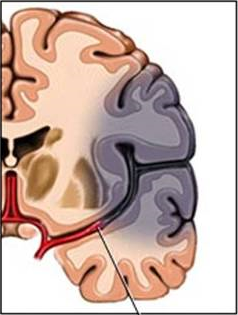
\includegraphics[width=0.5\textwidth]{isc_avc}
			\caption{AVC isquêmico}
			\label{fig:isq_avc}
		\end{subfigure}~
	\begin{subfigure}{0.5\textwidth}
			\centering
			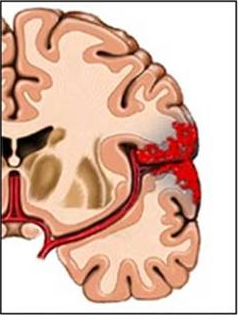
\includegraphics[width=0.5\textwidth]{hemo_avc}
			\caption{AVC hemorrágico}
			\label{fig:hemo_avc}
		\end{subfigure}
		\caption{Comparação entre os dois tipos de AVC}
	\end{figure}


	\subsection{Espasticidade}
	\paragraph{}"A espasticidade é uma desordem motora caracterizada por um aumento do tônus muscular [...] resultando da hiperexcitabilidade do reflexo de extensão".\cite{Lance80} Tônus muscular é a contração contínua e passiva do músculo, ou seja, o quão contraído o membro está quando em repouso.
	
	\begin{figure}[H]
		\centering
		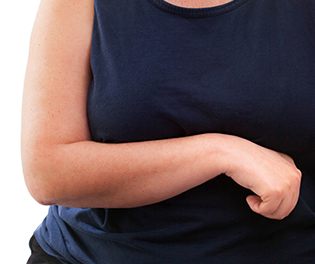
\includegraphics[width=0.5\textwidth]{spas_ex}
		\caption{Paciente com espasticidade}
		\label{fig:spasticity}
	\end{figure}
	
	\paragraph{}Este trabalho focará mais em espasticidade dos membros superiores (bíceps e tríceps). Para medir o grau da lesão, é utilizada a escala de Ashworth.
	
	\subsubsection{Escala de Ashworth}
	\paragraph{}A escala de Ashworth mede a resistência do movimento passivo, e é utilizada para quantificar o grau de espasticidade.
	
	\begin{table}[H]
		\centering
		\caption{Escala de Ashworth para Classificação da Espasticidade}
		\label{tab:ashworth}
	\begin{tabularx}{\textwidth}{|l X|}

		\hline
		\multicolumn{1}{|c}{Grau} & \multicolumn{1}{c|}{Descrição}                                                                                                            \\ \hline
		0                          & Nenhum aumento do tônus muscular                                                                                                          \\ \hline
		1                          & Pequeno aumento do tônus muscular, se expressando em uma minima resistência no final no movimento de extensão e flexão                    \\ \hline
		1+                         & Pequeno aumento do tônus muscular, se expressando em uma minima resistência em até metade do movimento de extensão e flexão               \\ \hline
		2                          & Médio aumento do tônus muscular, e uma resistência maior em grande parte do movimento de extensão e flexão, mas ainda move com facilidade \\ \hline
		3                          & Considerável aumento do tônus muscular, e dificuldade de realização do movimento de extensão e flexão                                     \\ \hline
		4                          & Grande aumento do tônus muscular, e as partes afetadas se tornam rígidas na extensão e flexão.\\ \hline
	\end{tabularx}
	\end{table}

\subsubsection{Escala de Rankin Modificada}

\paragraph{}A escala de Rankin\cite{Rankin57}, assim como a de Ashworth, mede a capacidade funcional do paciente acometido de AVC, a versão mais utilizada é a escala de Rankin modificada \cite{Swieten88}, que é uma escala de 6 pontos de simples classificação, indo desde falta total de sintomas, até a morte.

	\begin{table}[H]
	\centering
	\caption{Escala de Rankin Modificada}
	\label{tab:rankin}
	\begin{tabularx}{\textwidth}{|l X|}
		
		\hline
		\multicolumn{1}{|c}{Grau} & \multicolumn{1}{c|}{Descrição}                                                                                                            \\ \hline
		0                          & Nenhum sintoma e nenhuma limitação.                                                                                                          \\ \hline
		1                          & Sem deficiência motora apesar de possuir sintomas; pode executar todas as tarefas e atividades usuais.                    \\ \hline
		2                          & Deficiência leve; não pode executar todos as tarefas, mas consegue cuidar de suas necessidades básicas seu auxilio.\\ \hline
		3                          & Deficiência moderada; necessita de auxílio mas consegue andar sozinho.\\ \hline
		4                          & Deficiência forte; não consegue andar nem atender necessidades corporais sem auxílio.\\ \hline
		5                          & Deficiência severa; requer constante atenção e cuidado, acamado e incontinente. \\ \hline
	\end{tabularx}
\end{table}
	
	
	
	